\Chapter{Útvonalkereső heurisztikák}

\Section{Probléma felírása}

% útvonaltervezés, optimalizáció, keresési eljárások
Az alapvető cél, amit el szeretnénk érni, az találni egy optimális útvonalat, amely az akadályokat kikerülve eljuttatja a járművet valahová. Több megoldást is be fogok mutatni, az egyszerűbbektől a bonyolultabbakig. A kísérletek eredményei is láthatóak lesznek, melyek véletlenszerűen generált útvonalakat fognak ábrázolni bizonyos paraméterek alapján. Ezek után konkrét algoritmusokat fogok definiálni és bemutatni, melyek már tényleges optimumot adnak és adott kezdőpontból adott végpontba juttatják a járművet. 


\Section{Véletlen bolyongás}

Az első és legegyszerűbb (bár kevésbé hatékony) megoldás a véletlenszerű útvonalak generálása. Ennek lényege, hogy minél több útvonal közül ki tudja választani a gép azt, ami a legközelebb esik az elérni kívánt koordinátához vagyis a célhoz és nem ütközik egy akadályba sem, amelyek pozícióit mi határozzuk meg. Ezek definiálása a későbbiekben fog megtörténni.\\ 

\subsection{Útvonal generálás módszerei}

A véletlen útvonalakat jelen esetben úgy kell elképzelni, hogy a jármű kap bizonyos adatokat, hogy milyen szögben forduljon el adott időpillanatban. Tehát a kanyarodási szögek lesznek véletlenek és ezekből számítódnak majd az útvonalak. Elfordulás generálási módszer alapján figyelembe vehetünk két esetet:\\
\phantom{len}- abszolút elfordulás\\ 
\phantom{len}- relatív elfordulás\\
Abszolút elfordulás alatt azt értjük, hogy a generált szög lesz a jármű kanyarodási szöge, mindegy mi volt az előző elfordulás értéke. Relatív esetben pedig a generált szög mindig az előzőhöz adódik hozzá. Mindkét esetre láthatunk majd példákat, melyik megoldással milyen végpontokba juthatunk el vagy milyen útvonalakat kaphatunk. Be is mutatnám ezen paraméterek alapján az útvonal meghatározását és megvizsgálhatjuk az elérhető pontok eloszlását valamint valószínűségét.\\\\
Python program a relatív elfordulásos esetre:

\begin{python}
import math
from matplotlib import pyplot as plt
import random
\end{python}
Szükséges importok.

\begin{python}
def generate_random_angles_relative(number_of_turns):
        rel_angles = []
        angles = []
        for i in range(number_of_turns):
            angle = random.randint(-35, 35)
            angles.append(angle)
        for a in range(len(angles)):
            if a == 0:
                rel_angles.append(angles[0])
            else:
                rel_angles.append(angles[a])
                rel_angles[a] = angles[a] + rel_angles[a-1]
        return rel_angles
\end{python}
A függvény paraméterként az elfordulások számát várja. A belsejében pedig annyi random számot generál, amennyi ez az érték. A random szám alapértelmezett esetben -35 és +35, melyet az $angle$ változóba tárolok, majd hozzáadom őket egyesével egy listához. A maximum kanyarodási szög értéke sokmindentől függhet. A példában lévő szám egy teljesen átlagos elfordulási szögnek vehető egy személyautót tekintve. Szükséges lesz még egy for ciklus, amiben a generált szögeken végigmegyünk, majd az aktuális értékhez hozzáadjuk az előzőt (kivéve az elsőhöz). Így megkapjuk a kívánt értékeket. 

\begin{python}
rand_angles_rel = generate_random_angles_relative(30)
\end{python}
A függvény visszatérési értékét eltároljuk egy változóba. Paraméterként megadjuk, hogy hány kanyarodás történjen.

\begin{python}
def calc_path(pos_x, pos_y, steering_angles):
        path = []
        for deg in steering_angles:
            pos_x = pos_x + math.cos(math.radians(deg))
            pos_y = pos_y + math.sin(math.radians(deg))
            path.append((pos_x, pos_y))
        return path
\end{python}
A $calc\_path$ függvénnyel pedig az útvonalat tudjuk kiszámolni. Itt a kezdőpozíció $ x $ és $ y $ koordinátáit adhatjuk meg paraméterként, valamint a generált elfordulási szögeket, melyet a $rand\_angles\_rel$ változóban tárolunk. Itt is for ciklussal kell kiszámolnunk minden szögnél az adott pozíciót. Az aktuális pozícióhoz mindig hozzáadjuk az előzőt és az adott szög szinuszát és koszinuszát (annak függvényében, hogy $ x $ vagy $ y $ pozícióról van szó). 

\begin{python}
random_relative_path = calc_path(0, 0, rand_angles_rel)

x_random_relative = list(zip(*random_relative_path))[0]
y_random_relative = list(zip(*random_relative_path))[1]
\end{python}
A függvény meghívása, majd formázása a kirajzoláshoz. $ (x, y) $ alakról (tuple típusú változó) kell lebontani egy listába külön az $ x $ és külön az $ y $ értékeket. Ezt a $ zip $ funkcióval és a $ * $ operátor segítségével tehetjük meg.\\

\begin{python}
plt.plot(x_random_relative, y_random_relative, 'black')
plt.xlabel("x coordinates")
plt.ylabel("y coordinates")
plt.savefig('relative_example_path.png')
plt.show()
\end{python}
Ha pedig az eredményre vagyunk kíváncsiak, a $ matplotlib.pyplot $ könyvtár  $ plot() $ függvényét hívhatjuk meg, amely az x és y koordinátákat várja paraméternek és kirajzolja a grafikont. Ezzel kaptunk is egy példa útvonalat:

\begin{figure}[h!]
\centering
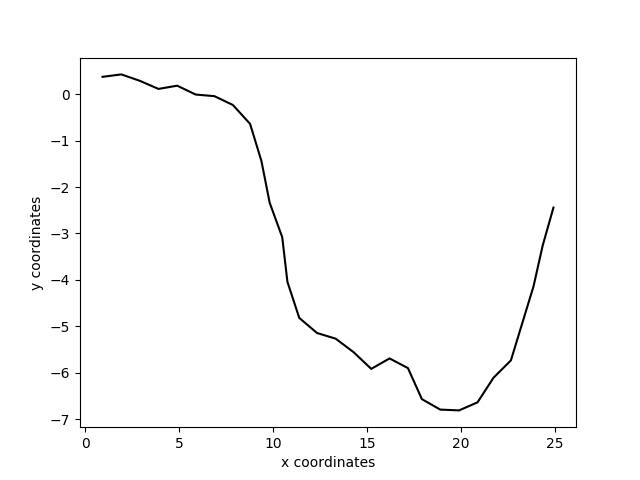
\includegraphics[scale=0.75]{images/relative_example_path.png}
\caption{Relatív random példa útvonal}
\label{fig:relative_path}
\end{figure}

Python program az abszolút elfordulásos esetre:

\begin{python}
def generate_random_angles_absolute(number_of_turns):
    random_angles = []
    for i in range(number_of_turns):
        angle = random.randint(-35, 35)
        random_angles.append(angle)
    return random_angles
    
def calc_path(pos_x, pos_y, steering_angles):
    path = []
    for deg in steering_angles:
        pos_x = pos_x + math.cos(math.radians(deg))
        pos_y = pos_y + math.sin(math.radians(deg))
        path.append((pos_x, pos_y))
    return path
    
rand_angles_absolute = generate_random_angles_absolute(30)

random_absolute_path = calc_path(0, 0, rand_angles_absolute)

x_random_absolute = list(zip(*random_absolute_path))[0]
y_random_absolute = list(zip(*random_absolute_path))[1]

plt.plot(x_random_absolute, y_random_absolute, 'blue')
plt.xlabel("x coordinates")
plt.ylabel("y coordinates")
plt.savefig('absolute_example_path.png')
plt.show()
\end{python}
Itt a generálás módja jóval egyszerűbb, ténylegesen csak egy random szám, amit nem ad hozzá az előző értékhez. Ez esetben az eredmény kevésbé reális, szinte minden útvonalban lesznek olyan szakaszok, ahol jelentős kólönbség van az előző és az aktuális szög között, így nagyobb törés figyelhető meg a vonalon.

\begin{figure}[h!]
\centering
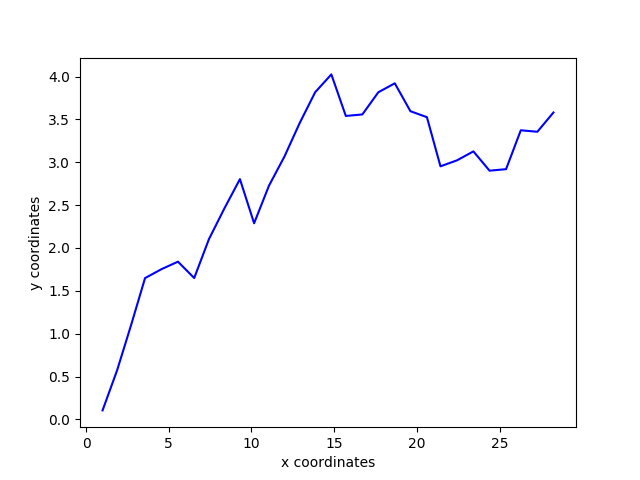
\includegraphics[scale=0.75]{images/absolute_example_path.png}
\caption{Abszolút random példa útvonal}
\label{fig:absolute_path}
\end{figure}


\newpage
\subsection{Ütközés detektálás véletlen útvonalak esetén}
Véletlen útvonalak esetén figyelmbe kell vennünk az esetleges akadályokat. Így a generált utak közül csak az lesz megfelelő, ami ezekbe nem ütközik bele. Tároljuk el ezeket mi magunk a programban, így létrehozva a környezetet. 

\begin{python}
obstacle1 = (2, 2, 6, 3)
obstacle2 = (8, 8, 6, 4)
obstacle3 = (15, 2, 4, 2)
obstacle4 = (8, -3, 4, 2)
obstacle5 = (23, -2, 4, 2)

obstacle_list = [obstacle1, obstacle2, obstacle3, obstacle4, obstacle5]
\end{python}
Paraméterek: obstacle(x1, y1, szélesség, magasság). Hozzáadjuk egy listához, hogy később azon végigiterálva meg tudjuk állapítani, hogy melyik obstacle objektumnál történt ütközés.

\begin{python}
def is_in_wall(x, y):
    collided = False
    collisions = []
    for index, obstacle in enumerate(obstacle_list):
        if obstacle[0] <= x <= (obstacle[0] + obstacle[2])\
                and obstacle[1] <= y <= (obstacle[1] + obstacle[3]):
            collisions.append((index, x, y))
            collided = True
    return collided, collisions
\end{python}
Az előző $ obstacle\_list $ listát végignézve ellenőrizzük, hogy az adott pont az akadály paraméterein belül esik-e. Ha igen, egy hamis változót igazra állítunk, valamint hozzáadjuk az adott pontot egy listához. Itt nem csak az $ x $ és $ y $ koordinátákat adom hozzá, hanem egy $ index $-et is, ami eltárolja, hogy melyik akadály objektumba ütközött az útvonal. Ha hamis, akkor a collided értéke is hamis marad. Visszatérünk két értékkel:

- volt-e ütközés

- az akadályba ütközött pontok listája

\begin{python}
def calc_path(pos_x, pos_y, steering_angles):
    path = []
    collisions = []
    for deg in steering_angles:
        pos_x = pos_x + math.cos(math.radians(deg))
        pos_y = pos_y + math.sin(math.radians(deg))
        if is_in_wall(pos_x, pos_y)[0]:
            collisions.append(is_in_wall(pos_x, pos_y)[1])
        path.append((pos_x, pos_y))
    return path, collisions
\end{python}
A már bemutatott $calc\_path$ függvényt kicsit átalakítva végig tudjuk nézni, hogy az útvonalon volt-e ütközés. Itt a for ciklus belsejében az adott pozíciót behelyettesítjük a függvény paraméterlistájába, és az első visszatérési értéket megadva feltételnek, ha az igaz, akkor hozzáadjuk az akadályba ütközött pontokat egy másik listához, amit a második visszatérési érték ad meg. Az útvonal minden eleme ugyanúgy bekerül a $ path $ listába. Majd szintén két értékkel térünk vissza:

- az útvonallal

- az akadályba ütközött pontokkal

\begin{python}
collision_list = []

def remove_nesting(nested_list):
    for i in nested_list:
        if type(i) == list:
            remove_nesting(i)
        else:
            collision_list.append(i)
            
random_relative_path_collisions = calc_path(0, 0, rand_angles_rel)[1]            
remove_nesting(random_relative_path_collisions)
\end{python}
Ezt a függvényt az akadályba ütközött pontok normalizálására hívom meg. Rekurzívan eltávolítja a listából a többi listát (bármennyi lehet egymásba ágyazva), így a későbbiekben egyszerűbben hivatkozhatunk a lista tuple típusú elemeire\\
($objektum\_index, x, y$). Az útvonal számító metódust meghívva, a második visszatérési értéke adja meg az ütközött pontokat.

\begin{python}
plt.figure()
rectangle1 = plt.Rectangle((2, 2), 6, 3, fc='blue', ec='red')
plt.gca().add_patch(rectangle1)
rectangle2 = plt.Rectangle((8, 8), 6, 4, fc='blue', ec='red')
plt.gca().add_patch(rectangle2)
rectangle3 = plt.Rectangle((15, 2), 4, 2, fc='blue', ec='red')
plt.gca().add_patch(rectangle3)
rectangle4 = plt.Rectangle((8, -3), 4, 2, fc='blue', ec='red')
plt.gca().add_patch(rectangle4)
rectangle5 = plt.Rectangle((23, -2), 4, 2, fc='blue', ec='red')
plt.gca().add_patch(rectangle5)

plt.plot(x_random_relative, y_random_relative, 'black')
plt.xlabel("x coordinates")
plt.ylabel("y coordinates")
plt.legend(collision_list, loc='upper left', bbox_to_anchor=(0, 1.17),
handletextpad=-0.1, handlelength=0)
plt.savefig('example_nocollision.png')
plt.show()
\end{python}
A listába szervezett akdályokat szemléltetés képpen rajzoljuk ki a területre a \\
$ matplotlib.patches.Rectangle $ funkciót használva. Majd a $ plot() $ függvénnyel az útvonalat kirajzolni, ha pedig volt ütközés, azt legendként jelenítem meg.\\\\
Ismét bemutatnék két példa útvonalat, amelyet a hivatkozott kódrészletek segítségével generáltam ezúttal akadályokkal. Néhány futtatás után kaptunk két hasonló útvonalat, az $ y $ végpontnál talán kissé több az eltérés. Ezt minél több próbálkozással (futtatással) lehetne optimalizálni. \\\\
A \ref{fig:example_nocollision} ábrán az útvonal látható, ahol nem volt ütközés. A \ref{fig:example_collision} ábrán pedig két objektumba is ütközött. Azokat az adatokat látjuk a legendben, ahol történt az ütközés. Az első elem, hogy melyik objektumba, a másik kettő pedig, hogy mely pontokban ütközött $ (x, y) $.

\begin{figure}[h!]
\centering
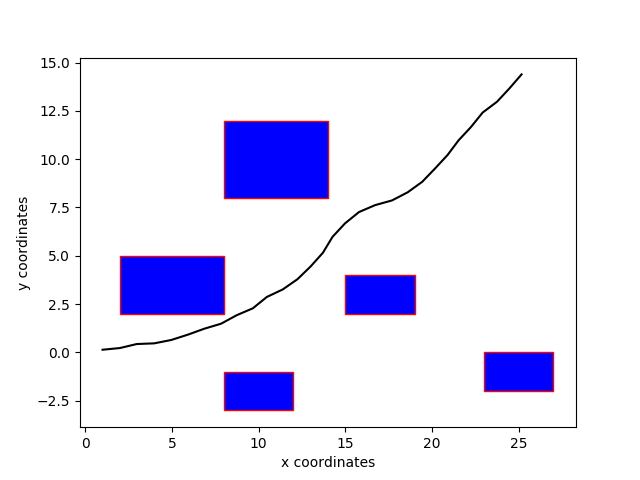
\includegraphics[scale=0.75]{images/example_nocollision.png}
\caption{Példa útvonal ütközés nélkül}
\label{fig:example_nocollision}
\end{figure}



\begin{figure}[h!]
\centering
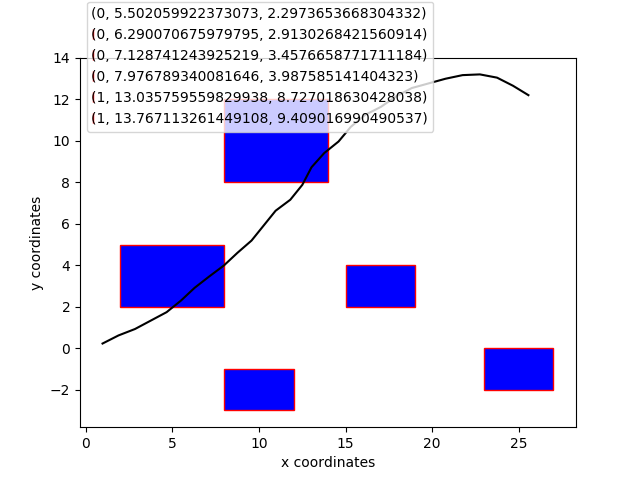
\includegraphics[scale=0.75]{images/example_collision.png}
\caption{Példa útvonal ütközéssel}
\label{fig:example_collision}
\end{figure}

 

\newpage
\subsection{Végpontok eloszlása, valószínűségi grafikonok}

Ebben az alpontban megvizsgáljuk, hogy különböző paraméterek esetén melyik pozícióba hány alkalommal, illetve milyen valószínűsággel juthatunk el. Legyen az alapértelmezett érték 10 000 mintaszám, tehát ennyi útvonalat fognak a függvények meghatározni. Kigyűjtöm a végpontok $ x $ és $ y $ koordinátáit 2 külön listába, ez alapján ábrázolható az értékek eloszlása.\\\\
Alap esetben legyen az elfordulások száma 30, kanyarodási szög -35$^{\circ}$, +35$^{\circ}$ közötti, generálás módszere relatív, a kezdőpozíció az origó (0, 0).\\\\
Ekkor a \ref{fig:no_obstacles_histogram2d} ábrán a (30, 0) körüli pozíciók a leggyakrabbak, de ugyanúgy gyakori eset például a (-11/+10, 28), melyek 70-70 gyakorisággal fordulnak elő.\\\\
A \ref{fig:obstacles_histogram2d} ábrán csak azokat a végpontokat látjuk, amikor nem volt egyáltalán ütközés. Ez minden esetben, 10 000 generálásnál 7000-7300 közötti rossz útvonalat számol, tehát átlagosan 2850 jó eredményből készül egy ilyen diagram. Az akadályok a \ref{fig:example_collision} vagy a \ref{fig:example_nocollision} ábrákon látható pozíciókban helyezkednek el ebben az esetben. Azt láthatjuk, hogy a leggyakoribb értékek a (12, -24/-26) pontokban lehetnek, szám szerint nagyjából 25-ször fordulnak elő. Tehát az y tengelyt tekintve inkább negatív irányba vinne minket a módszer, persze a pozitív értékeknél is léteznek útvonalak, de már csak 8-10 vagy kevesebb gyakorisággal. A világoskék színnel jelölt négyzetek is átlagban 10-szer, viszonylag gyakran fordulnak elő.



\begin{figure}[h!]
\centering
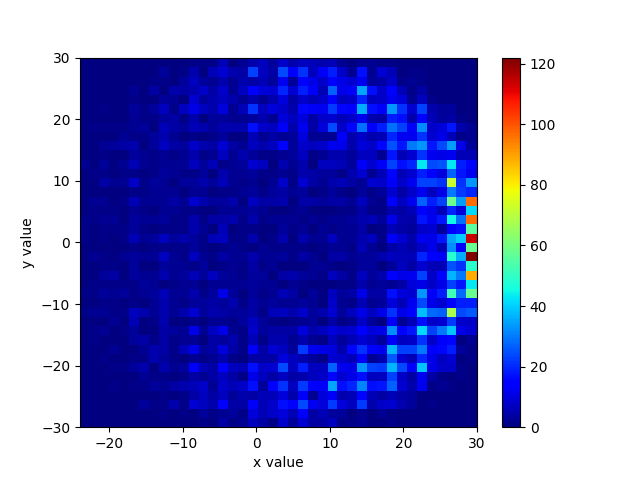
\includegraphics[scale=0.75]{images/no_obstacles_histogram2d.png}
\caption{Elérhető végpontok, ha nincs akadály a pályán}
\label{fig:no_obstacles_histogram2d}
\end{figure}

\begin{figure}[h!]
\centering
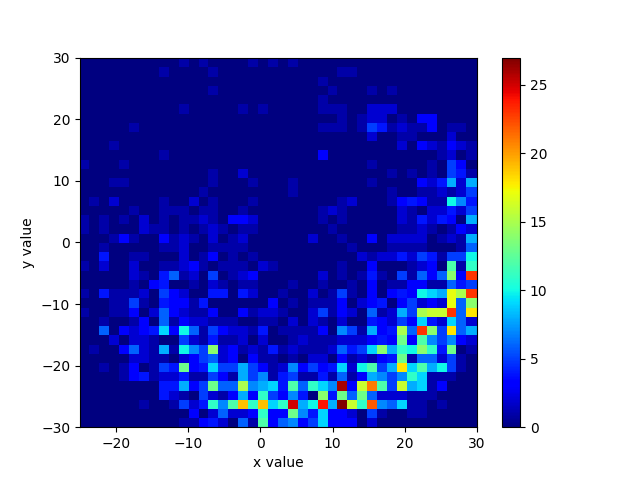
\includegraphics[scale=0.75]{images/obstacles_histogram2d.png}
\caption{Elérhető végpontok, ha vannak akadályok a pályán}
\label{fig:obstacles_histogram2d}
\end{figure}


\newpage

\Section{A* algoritmus}

\Section{Gépi tanítás a probléma inverzével}

% TODO: Véletlenszerű útvonalakhoz (mint jó megoldásokhoz) generálni akadályokat, és úgy tekinteni, hogy ez az algoritmus be- és kimenetére egy-egy példát jelent.
